\subsubsection{Relief valves}

\paragraph{Safety valves}

A safety valve is a valve that opens automatically when the pressure in the system exceeds a \ 
certain threshold. The resistance of a safety valve has the same form as for a standard valve, \ 
see equation \eqref{valve_resistance}, however the inverse loss coefficient $k_j^{-1}$ is given by
\begin{align}
    \boxed{ 
        k_j^{-1} = 
        \begin{cases}
            0, & \text{if } \Delta P_j \leq \Delta P_{\text{set}}, \\
            k_0^{-1}, & \text{if } \Delta P_j > \Delta P_{\text{set}},
        \end{cases}
    }
\end{align}
where $\Delta P_{\text{set}}$ is the set pressure difference at which the valve opens. This means \
that the safety valve is open when the pressure difference across it is greater than the set \
pressure difference and closed when the pressure difference is less than the set pressure \
difference. The value $k_0$ is the loss coefficient of the valve when it is fully open. For \
steady flow, the safety valve is considered to be closed $(\tau = 0)$, so the inverse loss \
coefficient is zero.

% Figure showing the valve open ratio as a function of pressure difference across the valve.
\begin{figure}
    \centering
    \begin{tikzpicture}[
        scale=1, 
        every node/.style={scale=0.8},
        greennode/.style={shape=rectangle, fill=green, draw=green, minimum size =0.01cm},
        rednode/.style={shape=rectangle, fill=red, draw=red, minimum size =0.01cm},
        blacknode/.style={shape=rectangle, fill=black, draw=black, minimum size =0.01cm},
    ] 
    \draw[thick, ->] (0,0) -- (0,3);
    \node[anchor=east] at (0,3) {$\tau$};
    \draw[thick, ->] (-2,0) -- (5,0);
    \node[anchor=north] at (5,0) {$\Delta P$};
    \node[anchor=north] at (3,-0.08) {$\Delta P_{\text{set}}$};
    \draw[fill=black] (3,0) circle (0.05cm);
    \node[anchor=east] at (0,2) {$1$};
    \node[anchor=north] at (0,0) {$0$};

    \draw[thick] (3,2) -- (5,2);
    \draw[thick] (3,2) -- (3,0);
    \draw[thick, dashed] (3,2) -- (0,2);

    \end{tikzpicture}
    \caption{Safety valve open ratio as a function of pressure difference across the valve.}
    \label{fig:safety_valve_open_ratio}
\end{figure}

\paragraph{Pressure relief valves}

Pressure relief valves are similar to safety valves, but they open more gradually as the pressure \
in the system increases. The resistance of a pressure relief valve has the same form as for a \
standard valve, see equation \eqref{valve_resistance}. For a pressure relief valve, the open ratio \ 
$\tau$ is a function of the pressure difference across the valve and is given by
\begin{align}
    \tau = \begin{cases}
        0, & \text{if } \Delta P_j \leq \Delta P_{\text{open}}, \\
        f(\Delta P_j), & \text{if } \Delta P_{\text{open}} < \Delta P_j < \Delta P_{\text{full}}, \\
        1, & \text{if } \Delta P_j \geq \Delta P_{\text{full}},
    \end{cases}
\end{align}
where $\Delta P_{\text{open}}$ is the pressure difference at which the valve starts to open, \
$\Delta P_{\text{full}}$ is the pressure difference at which the valve is fully open, and $f$ is a \
function that describes the profile of the valve opening. 

% Figure showing the valve open ratio as a function of pressure difference across the valve.
\begin{figure}
    \centering
    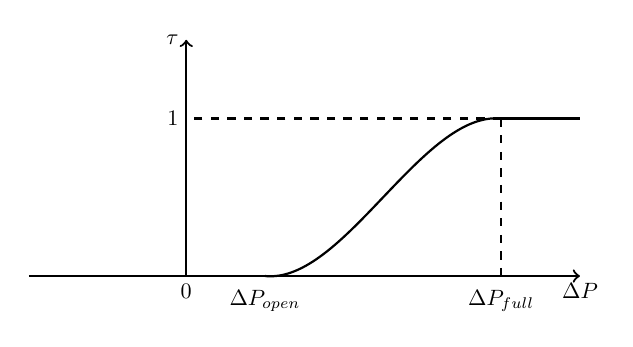
\begin{tikzpicture}[
        scale=1, 
        every node/.style={scale=0.8},
        greennode/.style={shape=rectangle, fill=green, draw=green, minimum size =0.01cm},
        rednode/.style={shape=rectangle, fill=red, draw=red, minimum size =0.01cm},
        blacknode/.style={shape=rectangle, fill=black, draw=black, minimum size =0.01cm},
    ] 
    \draw[thick, ->] (0,0) -- (0,3);
    \node[anchor=east] at (0,3) {$\tau$};
    \draw[thick, ->] (-2,0) -- (5,0);
    \node[anchor=north] at (5,0) {$\Delta P$};
    \node[anchor=north] at (4,-0.08) {$\Delta P_{\text{full}}$};
    \node[anchor=north] at (1,-0.08) {$\Delta P_{\text{open}}$};
    \node[anchor=east] at (0,2) {$1$};
    \node[anchor=north] at (0,0) {$0$};

    \draw[thick] (4,2) -- (5,2);
    \draw[thick, dashed] (4,2) -- (4,0);
    \draw[thick, dashed] (4,2) -- (0,2);

    \draw[thick] (1,0) .. controls (2,-0.1) and (3,2.1) .. (4,2);

    \end{tikzpicture}
    \caption{Pressure relief valve open ratio as a function of pressure difference across the valve.}
    \label{fig:pressure_relief_valve_open_ratio}
\end{figure}
